\section{Accuracy of current methods for predicting roll damping}
\label{se:accuracy_SI_method}
The most recognized and widespreadly used method to predict a ship's roll damping is the so-called simplified Ikeda's method. Some further development of the Ikeda's methods are also existed for specific ship types. However, these methods were seldom validated for wide ship applications due to for example lack of enough test data sources. Some studies also shows the simplified Ikeda's method is not capable to accurate predict the roll damping of modern ships. In the following, 227 existing roll decay model tests conducted at SSPA Maritime Dynamics Laboratory are used to check the accuracy of the simplified Ikeda's method and its extension methods. The comparison will help to identify the drawbacks and improvement potentials of the Ikeda's method. It aims at further developing this method to increase its accuracy based on the large test database through some statistical regression analysis.     

\subsection{Database of roll decay tests}
\label{se:database_of_roll_decay_tests}


Roll-decay model tests are normally performed prior to other dynamic tests, such as manoeuvring or seakeeping model tests, to check the properties of the tested ship model. In this study, results from such tests, carried out at SSPA in Sweden (www.sspa.se) have been used. The roll-decay tests are conducted by forcing the model to an initial roll angle and then releasing it to oscillate freely in six degrees of freedom. The tests are conducted either  at zero speed or at speed without autopilot. The scaled ship models are from 3 to 6 meters in  length. The measurement accuracy of these model tests is very good. When time series from 20 sets of repeated tests were investigated the average $R^2$ was found to be 0.995. The tests were originally conducted in connection with commercial projects for buildings new merchant ships. In this study, data collected from 2005 to 2018 were used to construct the roll-decay test database, which was applied to build a roll damping database. The ship types in the roll-decay tests used in this paper are  shown in Fig.\ref{fig:ship_types}, and the main parameters of these ships are presented in the sensitivity study as in Fig.\ref{fig:SI_sensitivity}. 


The parameter identification technique was used to estimate the roll damping coefficients from the roll-decay tests. It was investigated whether the linear model Eq.( \ref{eq:roll_decay_equation_himeno_linear}), quadratic model Eq.(\ref{eq:roll_decay_equation_himeno_quadratic_b}) or cubic model Eq.(\ref{eq:roll_decay_equation_cubic}) was best suited to describe the roll damping in all the tests to formulate the roll damping database. After the parameters were identified, the corresponding roll motions were simulated by the three mentioned models. The accuracy of the three models was evaluated with the $R^2$ score coefficient, based on model test and simulation time series of roll motions.
The average $R^2$ was 0.995 for the cubic model, 0.993 for the quadratic, and 0.986 for the linear model. In addition, Fig. \ref{fig:roll_decay_model_compare} shows a comparison between the models for one of the roll-decay tests. It can be seen that the linear model can not give a good representation of the whole range of roll motions, and the difference becomes obvious after the time of 30s. Since the quadratic model has almost the same accuracy as the cubic model it was selected to estimate roll damping from all the roll-decay tests in the database. All the extracted roll damping coefficients together with various ship related information will be formulated as the roll damping database for the following analysis.

\begin{figure}[H]
    \centering
    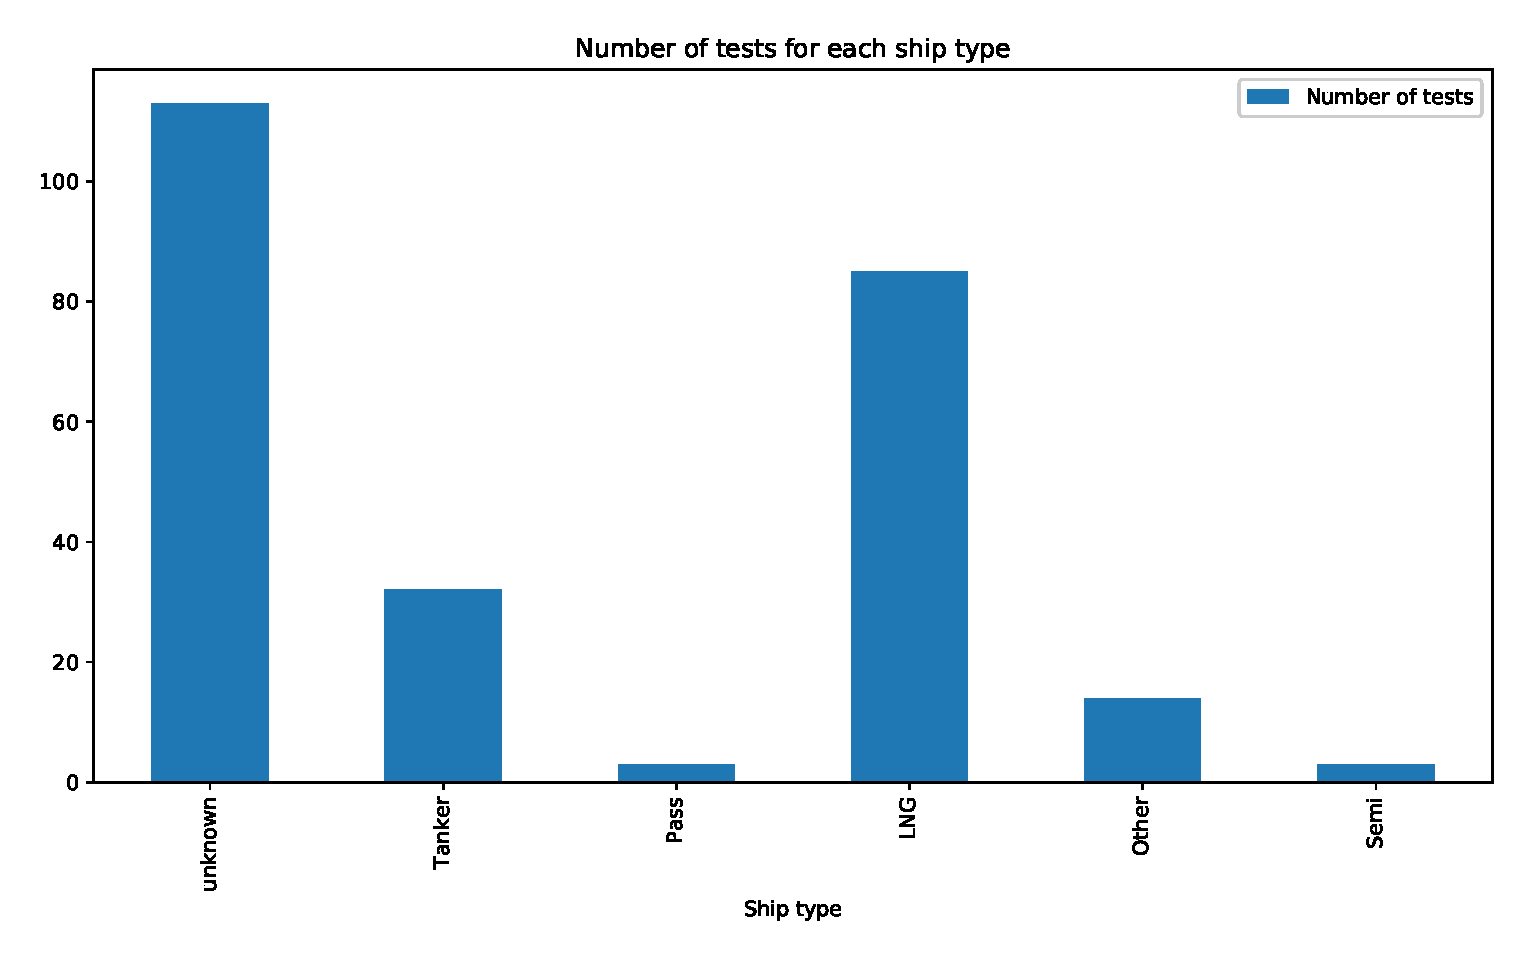
\includegraphics[width=0.5\columnwidth]{figures/ship_types.eps}
    \caption{Number of tests per ship type}
    \label{fig:ship_types}
\end{figure}

\begin{figure}[H]
    \centering
    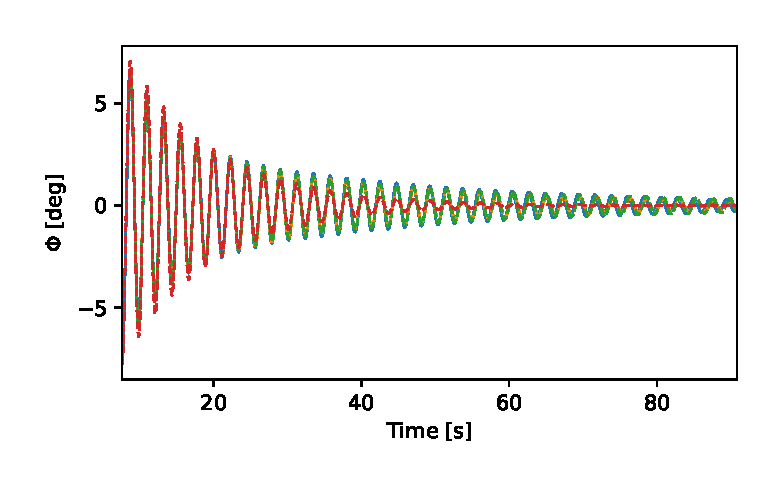
\includegraphics[width=12cm, height = 6cm ]{figures/roll_decay_model_compare.eps}
        \vspace{-0.5cm}
    \caption{Roll-decay test comparison of linear (bottom), quadratic (middle) and cubic model (upper).}
    \label{fig:roll_decay_model_compare}
\end{figure}
\subsection{Examples of damping estimation from tests}
\label{examples_damping_reference_fromdatabase}
In this section, we will present a few examples of model tests, and how the linear regression and nonlinear regression to give the accurate value of $B_e$, in comparison with the time series of motion response.

Note that: in \ref{se:Existing semi-empirical methods}, we only present the method to estimate the parameters, but no examples. Here we would like to prepare for some examples to confirm the way we are presented in \ref{se:Existing semi-empirical methods} is good enough to be acted as reference to regressed the improve Ikeda\'s method for semi-empirical damping ratio analysis.
\subsection{Overall accuracy of Simplified Ikeda method}
\label{se:overall_comparison}
%An investigation of how well the implementation of the SI-method agrees with the corresponding results in the roll damping database has been carried out. 
Comparing roll damping is a bit difficult since the roll damping model consist of two coefficients, a linear term $B_1$ and a quadratic term $B_2$. These coefficients can be combined by calculating the equivalent damping coefficient for a certain roll angle $\phi_a$ \parencite{himeno_prediction_1981}:

\begin{equation}
B_{e} = B_{1} + \frac{8 B_{2} \omega_{0} \phi_{a}}{3 \pi}
\end{equation}


For the roll damping database $B_1$ and $B_2$ can be inserted directly into Eq.(\ref{eq:B_e_equation}) to get the equivalent roll damping $B_e$. In order to obtain the same coefficients for the SI-method, roll damping was calculated for two roll amplitudes $\phi_a$ for the same motion frequency. $B_1$ and $B_2$ are obtained by fitting the Eq.(\ref{eq:B_e_equation}) to this data \parencite{himeno_prediction_1981}. The $B_e$ coefficient was made non-dimensional according to \parencite{himeno_prediction_1981}  giving the non-dimensional equivalent linear damping coefficient $\hat{B_e}$, which was more convenient to use for this comparison as follows,
\begin{equation} \label{eq:be_eqvalent}
    \hat{B_e} = \frac{B_e}{\rho \bigtriangledown Beam^2} \sqrt{\frac{Beam}{2g}},
\end{equation}
where $\rho$, $\bigtriangledown$ and $Beam$ stand for fluid density, displacement volume and breadth of a ship, respectively.
For the roll decay tests at SSPA, i.e., the database used in this study, the initial roll angle is normally set to 10 degrees, so that the model test data contain amplitudes in the range between 0 and 10 degrees. The root mean squared error of the equivalent roll damping, $RMSE_{\hat{B}_e}$, for various initial roll angles $\hat{B}_e(\phi_a)$ between estimation by the SI-method and the model test results is,

\begin{equation} \label{eq:rmse}
    RMSE({\hat{B}_e} (\phi_a)) = \sqrt{\frac{\sum\limits_{i=1}^n (\hat{B}_{e,i}^{SI} (\phi_a) - \hat{B}_{e,i}^{model} (\phi_a))^2}{n}},
\end{equation}
where $\hat{B}_{e,i}^{SI} (\phi_a)$ represents the equivalent roll damping by the SI-method for the i-th model test with initial roll angle of $\phi_a$, while $\hat{B}_{e,i}^{model} (\phi_a)$ represents the damping from the model tests. The results of the RMSE are plotted in the upper plot of Fig.\ref{fig:ikeda_phi_a}. Large values of $RMSE({\hat{B}_e})$ indicate very bad agreement between the SI-method and the model test results for roll damping prediction of modern ships. It should be noted that the accuracy decrease for larger amplitudes where nonlinear part of the SI-method plays a larger part. Furthermore, in order to illustrate the difference of $\hat{B}_e$ prediction between the SI-method and the model tests at SSPA, the three bottom plots of Fig.\ref{fig:ikeda_phi_a} presents the comparison for three roll amplitudes $\phi_a$ equal to 0, 5, 10 degrees, respectively. It shows that the accuracy differ very much between the amplitudes, with the highest accuracy at zero roll amplitude. 


\begin{figure}[H]
\centering
  \centering
  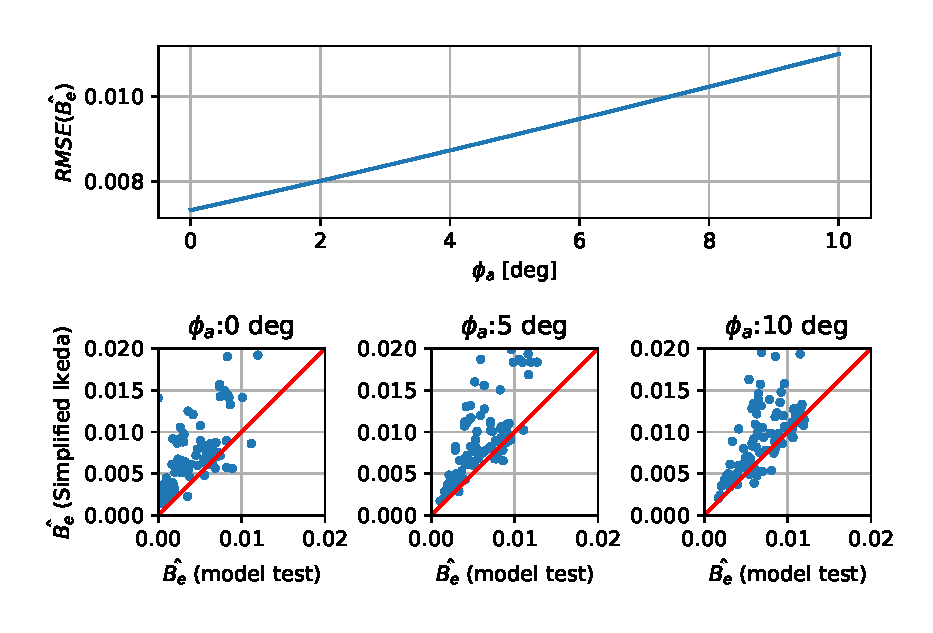
\includegraphics[]{figures/ikeda_phi_a.eps}
  \vspace{-0.5cm}
  \caption{Root mean square error of roll damping prediction between the SI-method and the model test results (upper plot). Influence of roll amplitude $\phi_a$ on $\hat{B_e}$ between the SI-method and model tests for $0^{\circ}$ (bottom left plot), $5^{\circ}$ (bottom middle plot) and $10^{\circ}$ (bottom right plot), respectively.}
  \label{fig:ikeda_phi_a}
\end{figure}

It was found that almost all ships in the roll damping database were outside the limits that are suitable to be applied in Eq.(\ref{eq:SI_limits}). Two different ways to handle this limit exceedance was investigated:
\begin{enumerate}
  \item the ``unlimited" approach where the input values are allowed to exceed the limits.
  \item the ``limited" approach where the limit boundary values were used for exceeding values.
\end{enumerate}

Fig.\ref{fig:ikeda_limited} show the comparison of roll damping predictions by the SI-method at 2 degrees roll amplitude, using the ``unlimited" and ``limited" approach with the corresponding results from model tests. The ``limited" approach seems to be the best one to use according to this figure, where the ``unlimited" approach has values very far away from the model test results (far away from the red reference line).   


\begin{figure}[H]
\vspace{-0.5cm}
\centering
  \centering
  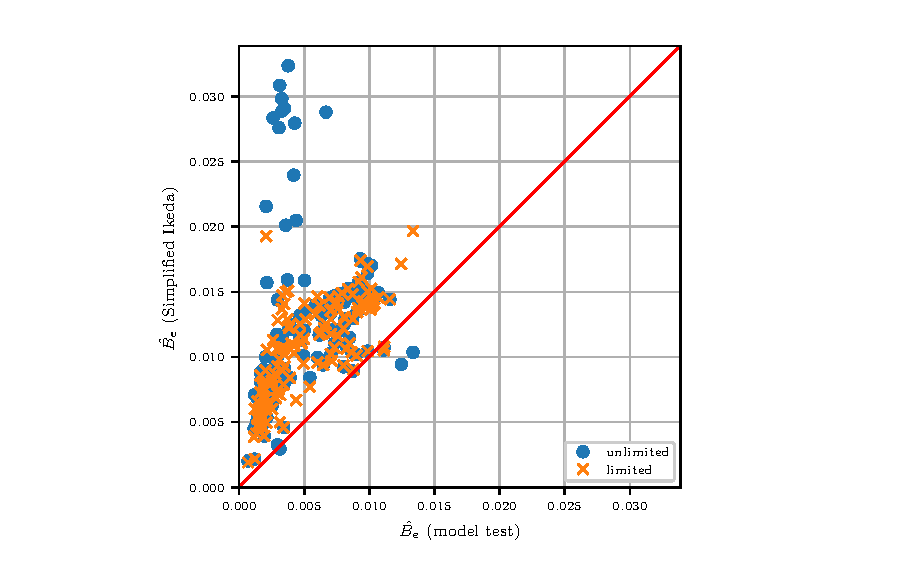
\includegraphics[]{figures/ikeda_limited.eps}
  \vspace{-0.5cm}
  \caption{$\hat{B_e}$ at all speeds estimated by the simplified Ikeda's method (Y-axis) in comparison with that from the roll decay test database (X-axis)}
  \label{fig:ikeda_limited}
\end{figure}
